%% 
%%	This is file 'beamer_sample.tex'
%%	according to an MPIDR's PowerPoint template (?)
%%	
%%	by Eric Naujoks
%%
%%	Problems, bugs and comments to 
%%	naujoks@demogr.mpg.de
%%

%%%%%%%%%%%%%%%%%%%%%%%%%%%%%%%%%%
%%	Praelegomena								%%
%%%%%%%%%%%%%%%%%%%%%%%%%%%%%%%%%%
%%	- Make sure that you use utf8-encoding for all your .tex-files!!! (TeXnicCenter since version 2.0)
%%	- TeXnicCenter update: MPIDR intranet > Hard- & Sortfware > Software > Script and text editors > TeXnicCenter

\documentclass[20pt,usenames,dvipsnames]{beamer}

\usepackage[ngerman,english]{babel}
\usepackage{tikz}
\usepackage[normalem]{ulem}
\geometry{paperwidth=10in, paperheight=7.5in}
\usepackage{animate}

\usepackage[utf8]{inputenc}

\usepackage[mpidr]{./mpidr/beamerthemeMPIDR}
%\usefonttheme{serif}
\newcolumntype{C}[1]{>{\centering\let\newline\\\arraybackslash\hspace{0pt}}m{#1}}
\newcommand*{\QEDA}{\hfill\ensuremath{\blacksquare}}
%% Declaring title and author
\title{Time spent and left of transient states in
stationary populations}
\subtitle{Tim Riffe \\ Francisco Villavicncio}		%%

%%	the institute's logo
\renewcommand{\mylogo}{\includegraphics[width=4.7in]{mpidr_logo_colour_en}}
\usepackage{color}
\definecolor{mygray}{rgb}{0.8,0.8,0.8}
\definecolor{yellow}{rgb}{1,1,0}

\defbeamertemplate{description item}{align left}{\insertdescriptionitem\hfill}
%%	should be the very last package to be loaded
\usepackage{hyperref}

%%%%%%%%%%%%%%%%%%%%%%%%%%%%%%%%%%
%%	Beginning of the document		%%
%%%%%%%%%%%%%%%%%%%%%%%%%%%%%%%%%%
\begin{document}

%%	titlepage - fixed frame:
%%	========================

% \begin{frame}
% 	\titlepage
% \end{frame}
\begin{frame}[plain]
	%\titlepage
	\vspace{-3cm}
 \centerline{\includegraphics[scale=.165]{beamerstrip3.png}}

	
	\huge
	\vspace{1em}
	
	Time spent and left of transient states in stationary populations\\
	\vspace{1em}
	\large 
	Tim Riffe \& Francisco Villavicencio \& Nicolas Brouard
\end{frame}
%-------------------


\begin{frame}[plain]
\Large
 \begin{block}{Brouard-Carey equality}
  Under stationarity, the population aged \textcolor{red}{$\mathbf{x}$} equals the population with \textcolor{blue}{$\mathbf{x}$} life left to live.\\ 
 \end{block}
\small{(Brouard, 1989; Vaupel, 2009; Villavicencio \& Riffe, 2016)}
\pause
\vspace{2em}
\Large
 \begin{block}{Transient equality}
  Under multistate stationarity, the probability that a randomly selected individual is in
  state \textcolor{OliveGreen}{$\mathbf{s}$} and entered
  \textcolor{OliveGreen}{$\mathbf{s}$} \textcolor{red}{$\mathbf{x}$} years ago
  is equal to the probability of being in state
  \textcolor{OliveGreen}{$\mathbf{s}$} and exiting in
  \textcolor{blue}{$\mathbf{x}$} years.
 \end{block}
\end{frame}

\begin{frame}[plain]
\Large
\centering
Requisites:
\begin{itemize}[<+->]
\item All vital and state transition schedules fixed.
\item No growth (births = deaths).
\item Result: The expected age-state structure is frozen.
\end{itemize}
\end{frame}


\begin{frame}[plain]
\Large
\begin{center}
\includegraphics[]{Figures/Proof0.pdf}
\end{center}
\end{frame}

\begin{frame}[plain]

\begin{center}
\includegraphics[]{Figures/Proof1.pdf}
\end{center}
\end{frame}

\begin{frame}[plain]
\Large
\begin{center}
\includegraphics[]{Figures/Proof2.pdf}
\end{center}
\end{frame}

\begin{frame}[plain]
\Large
\begin{center}
\includegraphics[]{Figures/Proof3.pdf}
\end{center}
\end{frame}

\begin{frame}[plain]
\Large
\begin{center}
\includegraphics[]{Figures/Proof4.pdf}
\end{center}
\end{frame}

\begin{frame}[plain]
\Large
\begin{center}
\includegraphics[]{Figures/Proof5.pdf}
\end{center}
\end{frame}

\begin{frame}[plain]
\Large
\begin{center}
\includegraphics[]{Figures/Proof6.pdf}
\end{center}
\end{frame}

\begin{frame}[plain]
\Large
\begin{center}
\includegraphics[]{Figures/Proof7.pdf}
\end{center}
\end{frame}

\begin{frame}[plain]
\Large
\begin{center}
\includegraphics[]{Figures/Proof8.pdf}
\end{center}
\end{frame}

\begin{frame}[plain]
\Large
\begin{center}
\includegraphics[]{Figures/Proof9.pdf}
\end{center}
\end{frame}

\begin{frame}[plain]
\Large
\begin{center}
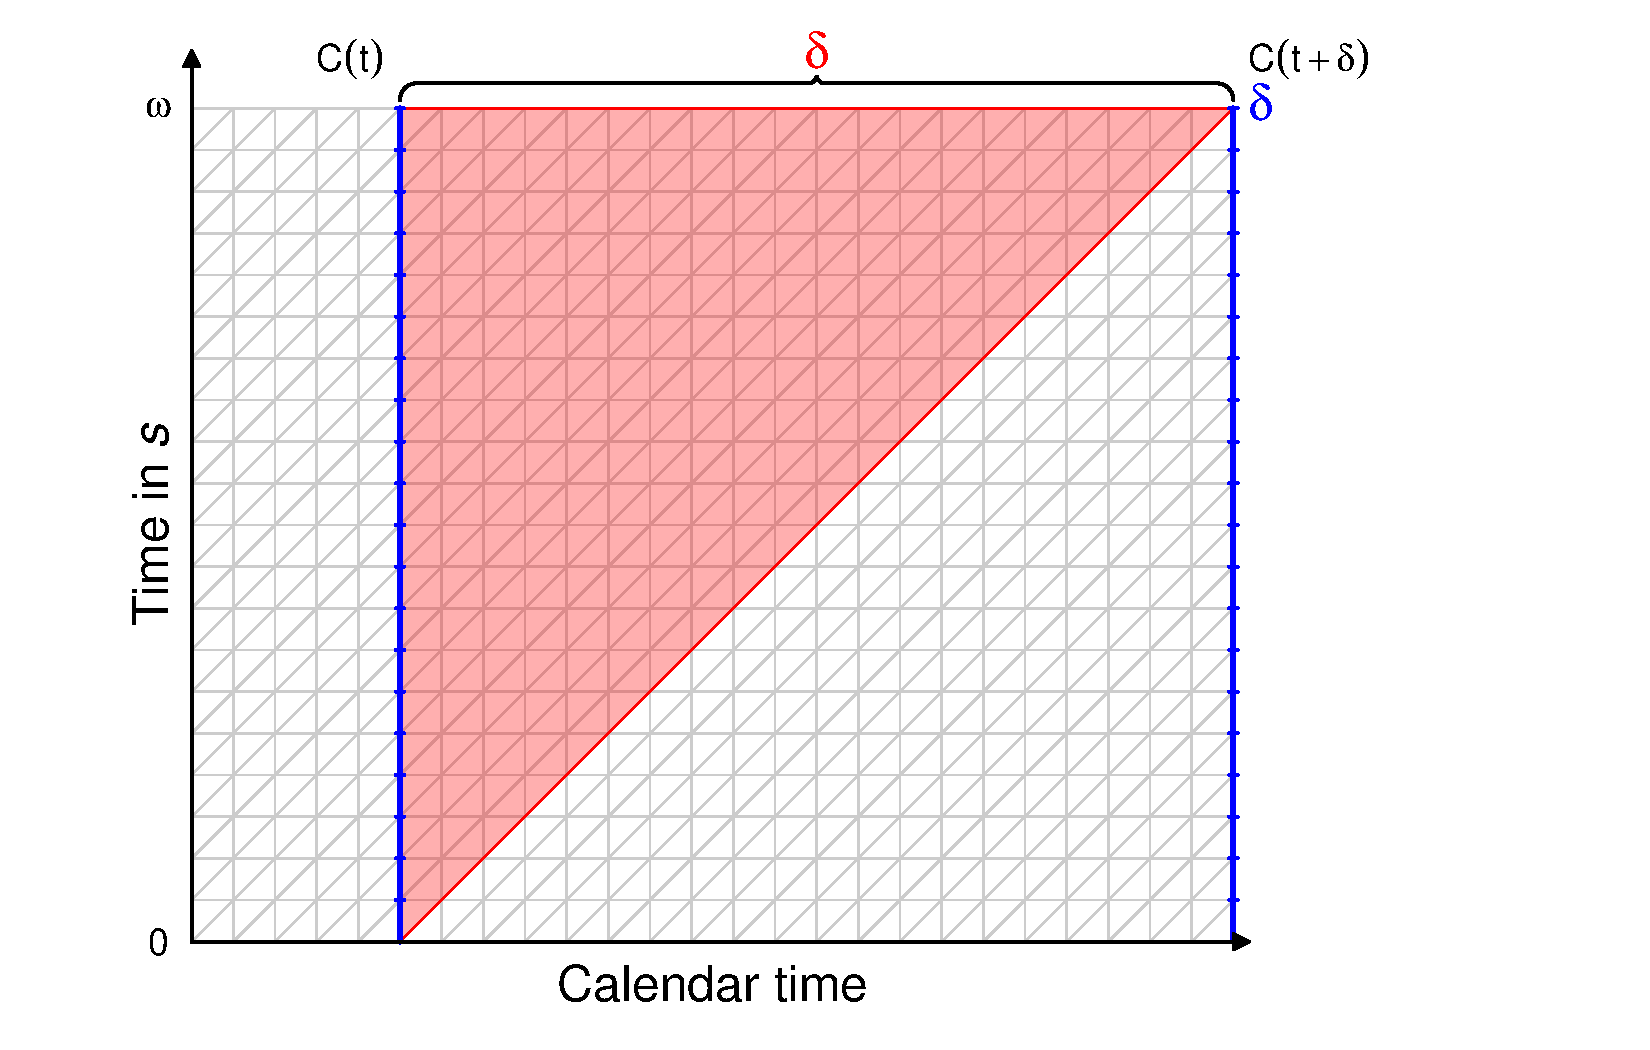
\includegraphics[]{Figures/Proof25.pdf}
\end{center}
\end{frame}

\begin{frame}[plain]
\Large
\begin{center}
\includegraphics[]{Figures/Symmetry.pdf}
\end{center}
\end{frame}


\begin{frame}[plain]
\Large
\begin{center}
Implications:
\pause
\begin{itemize}[<+->]
  \item Equal time spent-left distributions within states.
  \item Within episode \emph{order}. 
  \item Cumulative over episodes.
  \item Brouard-Carey is degenerate case.
\end{itemize}
\end{center}
\end{frame}

%
%% Now we install the new template for the following frames:
%{
%\usebackgroundtemplate{%
%  \includegraphics[width=\paperwidth,height=\paperheight]{Figures/eberhard-grossgasteiger-410620-unsplash.jpg}} 
%\begin{frame}[plain]
%\tiny
%\flushright
%\vspace{18cm}
%   Photo by Eberhard Grossgasteiger on Unsplash
%\end{frame}
%}


\usebackgroundtemplate{%
  \includegraphics[width=\paperwidth,height=\paperheight]{Figures/eberhard-grossgasteiger-410620-unsplash.jpg}} 
\begin{frame}[plain]
\Large
\centering
Might it be useful?
\tiny
\flushright
\vspace{16cm}
   Photo by Eberhard Grossgasteiger on Unsplash
\end{frame}

  
  \begin{frame}[plain]
\Large
\begin{center}
\pause
\begin{itemize}[<+->]
  \item High state turnover = shorter followup.
  \item Property observable in small stochastic samples. 
  \item Tractable under stability
\end{itemize}
\end{center}
\end{frame}
  
\begin{frame}
\vspace{9cm}
\Large
\begin{center}
Estimate from the reflection!\\ Thanks! \\
riffe@demogr.mpg.de
\end{center}
\end{frame}


%%%%%%%%%%%%%%%%%%%%%%%%%%%%%%%%%%
%%	End of the document			%%
%%%%%%%%%%%%%%%%%%%%%%%%%%%%%%%%%%
\end{document}



% Photo by eberhard grossgasteiger on Unsplash






